\documentclass[aspectratio=169]{beamer}

\usepackage{tikz}
\usetikzlibrary{shapes, backgrounds, arrows, positioning}
\usepackage{pgfplots}
\usepackage{listings}
\usepackage[utf8,latin1]{inputenc}
\usepackage[style = apa, backend = biber, natbib = true]{biblatex}
\addbibresource{../../literature/lit.bib}

\makeatletter \def\newblock{\beamer@newblock} \makeatother  

\beamertemplatenavigationsymbolsempty
\setbeamertemplate{itemize items}[circle]
\setbeamertemplate{section in toc}[circle]
\mode<beamer>{\setbeamercolor{math text displayed}{fg=iwmgray}}
\setbeamercolor{block body}{bg=iwmorange!50!white}
\setbeamercolor{block title}{fg=white, bg=iwmorange}

% Definitions for biblatex
\setbeamercolor{bibliography entry note}{fg=iwmgray}
\setbeamercolor{bibliography entry author}{fg=iwmgray}
\setbeamertemplate{bibliography item}{}

\definecolor{iwmorange}{RGB}{255,105,0}
\definecolor{iwmgray}{RGB}{67,79,79}
\definecolor{iwmblue}{RGB}{60,180,220}
\definecolor{iwmgreen}{RGB}{145,200,110}
\definecolor{iwmpurple}{RGB}{120,0,75}

\setbeamercolor{title}{fg=iwmorange}
\setbeamercolor{frametitle}{fg=iwmorange}
\setbeamercolor{structure}{fg=iwmorange}
\setbeamercolor{normal text}{fg=iwmgray}
\setbeamercolor{author}{fg=iwmgray}
\setbeamercolor{date}{fg=iwmgray}

\title{Simple and multiple linear regression}
\author{Nora Wickelmaier}
\date{Last modified: \today}

\lstset{language = R,%
  basicstyle = \ttfamily\color{iwmgray},
  frame = single,
  rulecolor = \color{iwmgray},
  commentstyle = \slshape\color{iwmgreen},
  keywordstyle = \bfseries\color{iwmgray},
  identifierstyle = \color{iwmpurple},
  stringstyle = \color{iwmblue},
  numbers = none,%left,numberstyle = \tiny,
  basewidth = {.5em, .4em},
  showstringspaces = false,
  emphstyle = \color{red!50!white}}

\pgfmathdeclarefunction{gauss}{2}{%
  \pgfmathparse{1/(#2*sqrt(2*pi))*exp(-((x-#1)^2)/(2*#2^2))}%
}

\AtBeginSection[]{
  \frame{
    \tableofcontents[sectionstyle=show/hide, subsectionstyle=show/show/hide]}}

\setbeamertemplate{headline}{
 \begin{beamercolorbox}{section in head}
   \vskip5pt\insertsectionnavigationhorizontal{\paperwidth}{}{}\vskip2pt
 \end{beamercolorbox}
}

\setbeamertemplate{footline}{\vskip-2pt\hfill\insertframenumber$\;$\vskip2pt}

\begin{document}

\begin{frame}{}
\thispagestyle{empty}
\titlepage
\end{frame}

\begin{frame}{Outline}
\tableofcontents
\end{frame}


\begin{frame}{What is regression?}
  \pause
  Set of statistical processes for estimating the relationships between a
  dependent variable (often called the `outcome variable') and one or more
  independent variables (often called `predictors', `covariates', or
  `features')
  \flushright{\tiny{\url{https://en.wikipedia.org/wiki/Regression_analysis}}}
  \pause
\vfill
  \begin{itemize}
    \item Predict an outcome variable
    \item Compare predictions for different groups
    \item ``Find the line that most closely fits the data''
    \item Continuous outcome $y$
  \end{itemize}
\end{frame}

\section{Basic concepts}

\begin{frame}{Simple linear regression}
\begin{columns}
\begin{column}{.5\textwidth}
  \begin{itemize}
    \item For the pairs
      \[
        (x_1, y_1), \ldots, (x_n, y_n),
      \]
    we get the stochastical model
      \begin{align*}
        y_i & = \beta_0 + \beta_1 \cdot x_i + \varepsilon_i\\
        \varepsilon_i & \sim N(0, \sigma^2)~\text{i.i.d.}
      \end{align*}
    for all $i = 1, \dots, n$
    \item Errors are independent identically distributed (i.i.d.)
  \end{itemize}
\end{column}
\begin{column}{.5\textwidth}
  % Created by tikzDevice version 0.6.2-92-0ad2792 on 2012-11-14 12:23:43
% !TEX encoding = UTF-8 Unicode
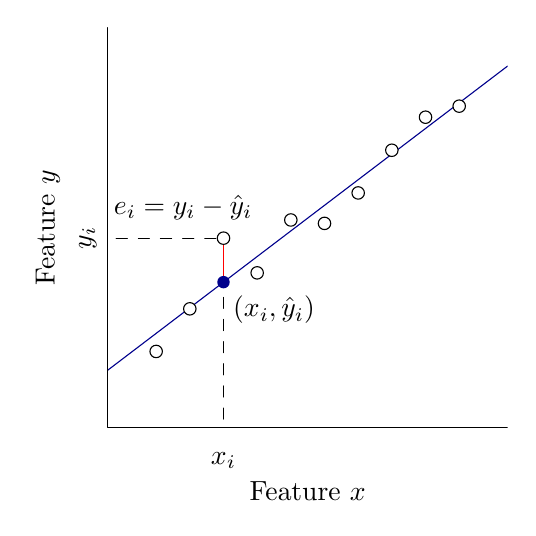
\begin{tikzpicture}[x=1pt,y=1pt]
\definecolor[named]{fillColor}{rgb}{1.00,1.00,1.00}
\path[use as bounding box,fill=fillColor,fill opacity=0.00] (0,0) rectangle (173.45,173.45);
\begin{scope}
\path[clip] (  0.00,  0.00) rectangle (173.45,173.45);
\definecolor[named]{drawColor}{rgb}{0.00,0.00,0.00}

\node[text=drawColor,anchor=base,inner sep=0pt, outer sep=0pt, scale=
  1.00] at (101.18,  2.51) {Feature $x$};

\node[text=drawColor,rotate= 90.00,anchor=base,inner sep=0pt, outer
  sep=0pt, scale=  1.00] at (  9.71,101.18) {Feature $y$};
\end{scope}
\begin{scope}
\path[clip] ( 28.91, 28.91) rectangle (173.45,173.45);
\definecolor[named]{drawColor}{rgb}{0.00,0.00,0.55}

\path[draw=drawColor,line width= 0.4pt,line join=round,line cap=round] ( 28.91, 49.66) -- (173.45,159.60);
\definecolor[named]{drawColor}{rgb}{0.00,0.00,0.00}

\path[draw=drawColor,line width= 0.4pt,dash pattern=on 4pt off 4pt ,line join=round,line cap=round] (  0.00, 97.39) --
	( 70.76, 97.39);

\path[draw=drawColor,line width= 0.4pt,dash pattern=on 4pt off 4pt ,line join=round,line cap=round] ( 70.76,  0.00) --
	( 70.76, 81.50);
\definecolor[named]{drawColor}{rgb}{1.00,0.00,0.00}

\path[draw=drawColor,line width= 0.4pt,line join=round,line cap=round] ( 70.76, 81.50) --
	( 70.76, 97.39);
\definecolor[named]{fillColor}{rgb}{0.00,0.00,0.55}

\path[fill=fillColor] ( 70.76, 81.50) circle (  2.25);
\definecolor[named]{drawColor}{rgb}{0.00,0.00,0.00}
\definecolor[named]{fillColor}{rgb}{1.00,1.00,1.00}

\path[draw=drawColor,line width= 0.4pt,line join=round,line cap=round,fill=fillColor] ( 46.43, 56.45) circle (  2.25);

\path[draw=drawColor,line width= 0.4pt,line join=round,line cap=round,fill=fillColor] ( 58.59, 71.85) circle (  2.25);

\path[draw=drawColor,line width= 0.4pt,line join=round,line cap=round,fill=fillColor] ( 70.76, 97.39) circle (  2.25);

\path[draw=drawColor,line width= 0.4pt,line join=round,line cap=round,fill=fillColor] ( 82.93, 84.85) circle (  2.25);

\path[draw=drawColor,line width= 0.4pt,line join=round,line cap=round,fill=fillColor] ( 95.09,103.96) circle (  2.25);

\path[draw=drawColor,line width= 0.4pt,line join=round,line cap=round,fill=fillColor] (107.26,102.73) circle (  2.25);

\path[draw=drawColor,line width= 0.4pt,line join=round,line cap=round,fill=fillColor] (119.43,113.73) circle (  2.25);

\path[draw=drawColor,line width= 0.4pt,line join=round,line cap=round,fill=fillColor] (131.59,129.16) circle (  2.25);

\path[draw=drawColor,line width= 0.4pt,line join=round,line cap=round,fill=fillColor] (143.76,141.10) circle (  2.25);

\path[draw=drawColor,line width= 0.4pt,line join=round,line cap=round,fill=fillColor] (155.93,145.09) circle (  2.25);

\node[text=drawColor,anchor=base,inner sep=0pt, outer sep=0pt, scale=  1.00] at ( 89.01, 68.94) {$(x_i, \hat{y}_i)$};

\node[text=drawColor,anchor=base,inner sep=0pt, outer sep=0pt, scale=  1.00] at ( 56.16,106.11) {$e_i = y_i - \hat{y}_i$};
\end{scope}
\begin{scope}
\path[clip] (  0.00,  0.00) rectangle (173.45,173.45);
\definecolor[named]{drawColor}{rgb}{0.00,0.00,0.00}

\node[text=drawColor,anchor=base,inner sep=0pt, outer sep=0pt, scale=  1.00] at ( 70.76, 15.71) {$x_i$};

\node[text=drawColor,rotate= 90.00,anchor=base,inner sep=0pt, outer sep=0pt, scale=  1.00] at ( 22.91, 97.39) {$y_i$};

\path[draw=drawColor,line width= 0.4pt,line join=round,line cap=round] ( 28.91,173.45) --
	( 28.91, 28.91) --
	(173.45, 28.91);
\end{scope}
\end{tikzpicture}

\end{column}
\end{columns}
\end{frame}

\begin{frame}{Simple linear regression}
  \begin{itemize}
    \item From the properties of the error variables, we conclude
\[
  E(y_i) = E(\beta_0 + \beta_1 \cdot x_i + \varepsilon_i) =
  \beta_0 + \beta_1 \cdot x_i = \bar{y}
\]
and
\[
  Var(y_i) = Var(\beta_0 + \beta_1 \cdot x_i + \varepsilon_i) = \sigma^2
\]
\item For a given $x_i$, the stochastical independence of $\varepsilon_i$
  transfers to $y_i$\\[2ex]
  \end{itemize}
\end{frame}

\begin{frame}{Parameter estimation}
  \begin{itemize}
    \item The parameters $\beta_0$ and $\beta_1$ are estimated with the method
      of least squares
    \item Hereby, the sum of squares of the residuals is minimized
      \[
        \sum_{i=1}^n \varepsilon_i^2
        = \sum_{i=1}^n (y_i - \hat{y}_i)^2
        = \sum_{i=1}^n (y_i - \beta_0 - \beta_1 \, x_i)^2
        = \text{min}
      \]
    \item The minimum is obtained by setting the partial derivatives for
      $\beta_0$ and $\beta_1$ to 0
      \[
        \frac{\partial \left( \sum_{i=1}^n (y_i - \beta_0 - \beta_1 \, x_i)^2\right)}
        {\partial \beta_0}  ~~~~~
        \frac{\partial \left( \sum_{i=1}^n (y_i - \beta_0 - \beta_1 \, x_i)^2\right)}
        {\partial \beta_1} 
      \]
    \item Solving these equations results in
      \[
        \hat\beta_0 = \bar y - \hat\beta_1 \bar x ~~~~~ \text{and} ~~~~~
        \hat\beta_1 = \frac{\sigma_{xy}}{\sigma^2_{x}}
      \]
      where $\sigma_{xy}$ is the covariance between $x$ and $y$
  \end{itemize}
\end{frame}

\begin{frame}{Correlation coefficient}
  \begin{itemize}
    \item The correlation coefficient $r$ is defined as the standardized
      covariance
      \[
        r = \frac{\sigma_{xy}}{\sigma_x \sigma_y}
      \]
    \item Hence, we get
      \[
        \hat\beta_1 = \frac{\sigma_{y}}{\sigma_x} r
      \]
    \item When $x$ and $y$ are $z$ standardized with $\bar x = \bar y = 0$ and
      $\sigma_x = \sigma_y = 1$, we get
      \[
        \hat\beta_0 = 0 ~~~~~ \text{and} ~~~~~ \hat\beta_1 = r
      \]
  \end{itemize}
\end{frame}

\begin{frame}{Determination coefficient}
  \begin{itemize}
    \item With the assumptions made so far, it can be shown that the variance of
      the residuals
      \[
      \sigma_{\varepsilon}^2 = \frac{1}{n}\sum_{i=1}^n (y_i - \hat y_i)^2
      \]
      can be rewritten as
      \[
        \sigma_{\varepsilon}^2 = (1 - r^2) \sigma_y^2
      \]
    \item The factor $(1 - r^2)$ determines the proportion of the variance of
      $y$ that cannot be explained by the regression of $x$
    \item Hence, he determination coefficient $r^2$ gives the proportion of the
      variance of $y$ explained by $x$
      \[
        r^2 = \frac{\sigma_{\hat y}^2}{\sigma_{y}^2}
      \]
  \end{itemize}
\end{frame}

\begin{frame}{Variance decomposition}
\begin{columns}[c]
\begin{column}{6cm}
  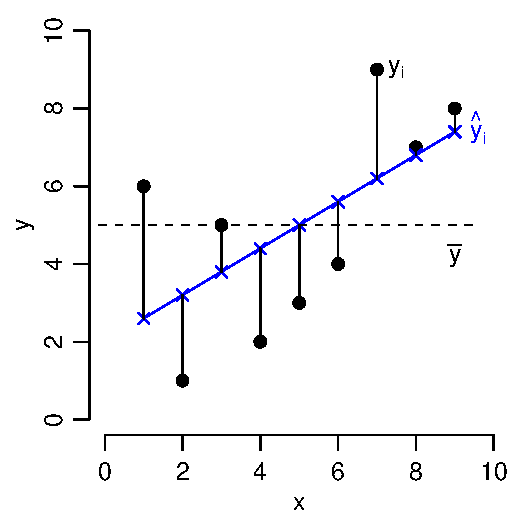
\includegraphics[scale=.7]{../figures/obs_pred}
\end{column}
%
\begin{column}{5cm}
{\small
\[
  \sigma_y^2 = \sigma_{\hat y}^2 + \sigma_e^2
\]
\[
  \frac{1}{n} \sum_{i=1}^n (y_i - \bar{y})^2 =
\]
\[
  \frac{1}{n} \sum_{i=1}^n (\hat{y_i} - \bar{y})^2 +
  \frac{1}{n} \sum_{i=1}^n (y_i - \hat{y_i})^2
\]
}
\end{column}
\end{columns}
\vfill
\end{frame}

\begin{frame}{}
  \begin{block}{Exercise}
    \begin{itemize}
      \item Simulate a data set based on a simple regression model with
        \begin{align*}
          \beta_0 & = 0.2\\
          \beta_1 & = 0.3\\
          \sigma & = 0.5\\
          x & \in [1, 20]~\text{in steps of 1}
        \end{align*}
        \vspace{-.5cm}
      \item What functions in $R$ do we need?
    \end{itemize}
  \end{block}
\end{frame}

\begin{frame}[fragile]{Simulate data set}
\begin{lstlisting}
x     <- 1:20
n     <- length(x)
a     <- 0.2
b     <- 0.3
sigma <- 0.5
y     <- 0.2 + 0.3 * x + rnorm(n, sd = sigma)

dat <- data.frame(x, y)

# clean up workspace
rm(x, y)

# plot data
plot(y ~ x, data = dat)
\end{lstlisting}
  \nocite{GelmanHill2020}
\end{frame}

\begin{frame}[fragile]{Fit regression model}
\begin{lstlisting}
lm1 <- lm(y ~ x, data = dat)
summary(lm1)

mean(resid(lm1))
sd(resid(lm1))
hist(resid(lm1), breaks = 15)

# plot data
plot(y ~ x, data = dat)
abline(lm1)
\end{lstlisting}
\end{frame}

\begin{frame}[fragile]{Re-cover parameters}
\begin{lstlisting}
pars <- replicate(2000, {
  ysim <- 0.2 + 0.3 * x + rnorm(n, sd = sigma)
  lm1  <- lm(ysim ~ x, data = dat)
  c(coef(lm1), sigma(lm1))
})

rowMeans(pars)
# standard errors
apply(pars, 1, sd)

hist(pars[1, ])
hist(pars[2, ])
hist(pars[3, ])
\end{lstlisting}
\end{frame}

\begin{frame}{Sample distribution}
  \begin{center}
  \begin{tikzpicture}
\begin{axis}[every axis plot post/.append style={
  mark=none, domain=-4:4, samples=50, smooth},
    % All plots: from -2:2, 50 samples, smooth, no marks
  axis x line*=bottom, % no box around the plot, only x and y axis
  axis y line*=left,   % the * suppresses the arrow tips
  enlargelimits=upper] % extend the axes a bit to the right and top
\addplot[color=iwmorange, fill=iwmorange!50] {gauss(0, 1)};
%\addplot[color=iwmgray, fill=iwmgray!50, opacity=.5] {gauss(3, 1)};
\draw (axis cs: 0, 0) -- (axis cs: 0, .4);
  \draw[dashed] (axis cs: 0, .241) -- (axis cs: 1, .241);
  \draw[dashed] (axis cs: 1, 0) -- (axis cs: 1, .241);
\node[color=iwmorange] at (axis cs: 0, .42) {$\theta$};
  \node[color=iwmgray]   at (axis cs: 1.4, .241) {$se$};
\end{axis}
\end{tikzpicture}
  \end{center}
\end{frame}

\begin{frame}{}
  \begin{block}{Exercise}
    \begin{itemize}
      \item Simulate data with the parameters from slide~11
      \item Do not assume that we have one subject per value for $x$, but
        more than one subject
      \item Simulate data for $n=40$ and $n=100$\\
        Hint: Use \texttt{sample(x, n, replace = TRUE)}
      \item Re-cover your parameters as done on slide~14
      \item What happens to your standard errors?
    \end{itemize}
  \end{block}
\end{frame}

\begin{frame}{Confidence intervals}
  \begin{itemize}
    \item We get the $(1-\alpha)$ confidence intervals for the estimates with
\[
  \left[\hat{\beta_0} - \hat{\sigma}_{\hat{\beta_0}} \, t_{1-\alpha/2} (n-2),~
  \hat{\beta_0} + \hat{\sigma}_{\hat{\beta_0}} \, t_{1-\alpha/2} (n-2)\right]
\]
and
\[
  \left[\hat{\beta_1} - \hat{\sigma}_{\hat{\beta_1}} \, t_{1-\alpha/2} (n-2),~
  \hat{\beta_1} + \hat{\sigma}_{\hat{\beta_1}} \, t_{1-\alpha/2} (n-2)\right]
\]
  \item For $n > 30$ the $t$ quantiles of the $t(n-2)$ distribution can be
    replaced by quantiles of the $N(0,1)$ distributiom

  \item For a sufficient sample size, even when the normality assumption is
    violated, the least square estimators is approximately $t$ or normally
      distributed
  \end{itemize}
\end{frame}

\begin{frame}[fragile]{Hypothesis tests}
  {Wald test}
  \begin{itemize}
    \item The estimates for $\beta_0$ and $\beta_1$ are unbiased, sufficient,
      consistent, and efficient
    \item The normality assumption implies
\[
  \hat{\beta_0} \sim N (\beta_0, \sigma^2_{\hat{\beta_0}})
  ~~~\text{and}~~~
  \hat{\beta_1} \sim N (\beta_1, \sigma^2_{\hat{\beta_1}})
\]
      and with that for some hypothetical value $\gamma_0$
\[
  T_{\beta_0} = \frac{\hat{\beta_0} - \gamma_0}{\hat{\sigma}_{\hat{\beta_0}}} \sim t (n-2)
  ~~~\text{und}~~~
  T_{\beta_1} = \frac{\hat{\beta_1} - \gamma_0}{\hat{\sigma}_{\hat{\beta_1}}} \sim t (n-2)
\]
with estimates $\hat{\sigma}^2_{\hat{\beta_0}}$ and
$\hat{\sigma}^2_{\hat{\beta_1}}$ for the variances
    \item We are usually interested in the hypotheses $\beta_0 = 0$ and $\beta_1
      = 0$, hence $\gamma_0 = 0$ and
\[
  T_{\beta_0} = \frac{\hat{\beta_0}}{\hat{\sigma}_{\hat{\beta_0}}} \sim t (n-2)
  ~~~\text{und}~~~
  T_{\beta_1} = \frac{\hat{\beta_1}}{\hat{\sigma}_{\hat{\beta_1}}} \sim t (n-2)
\]
  \end{itemize}
\end{frame}

\begin{frame}{Overall $F$ test}
  \begin{itemize}
    \item For simple linear regression, we can construct an equivalent test
      for testing $\beta_1 = 0$ using variance decomposition
    \item This test can conceptionally be considered to test, if predictor $x$
      explains a significant proportion of the variance of $y$
\[
  F = \dfrac{~~\dfrac{\sum_{i=1}^n (\hat{y}_i - \bar{y})^2}{1}~~}
      {\dfrac{\sum_{i=1}^n (y_i - \hat{y}_i)^2}{n-2}} = 
      \dfrac{R^2}{1 - R^2} \, (n - 2)
\]
\item It can be shown that $F = T^2-{\gamma_0}$ for $\gamma_0 = 0$
 with $F \sim F(1,n-2)$
 \item With this more general test, we can also test the assumption that any
   variance of $y$ is explained by the predictors in a multiple regression 
  \end{itemize}
\end{frame}

\section{Assumptions}

\begin{frame}{Assumptions}
  \begin{itemize}
    \item We have the stochastic model $y_i = \beta_0 + \beta_1 \cdot x_i +
      \varepsilon_i$ with $\varepsilon_i \sim N(0, \sigma^2)~\text{i.i.d.}$
    \item The error variables $\varepsilon_i$ are considered to be
      non-observable and comprise influence that cannot be controlled and is
      unsystematic (or random)
    \item Hence, it makes sense to assume
    \[
      E(\varepsilon_i) = 0, ~\text{for all}~ i = 1, \ldots, n
    \]
    and
    \[
      Var(\varepsilon_i) = \sigma^2, ~\text{for all}~ i = 1, \ldots, n
    \]
  \item From this follows
\[
  E(y_i) = E(\beta_0 + \beta_1 \cdot x_i + \varepsilon_i) =
  \beta_0 + \beta_1 \cdot x_i
\]
and
\[
  Var(y_i) = Var(\beta_0 + \beta_1 \cdot x_i + \varepsilon_i) = \sigma^2
\]
  \end{itemize}
\end{frame}

\begin{frame}{Assumptions}
  \begin{columns}
    \column{.6\textwidth}
    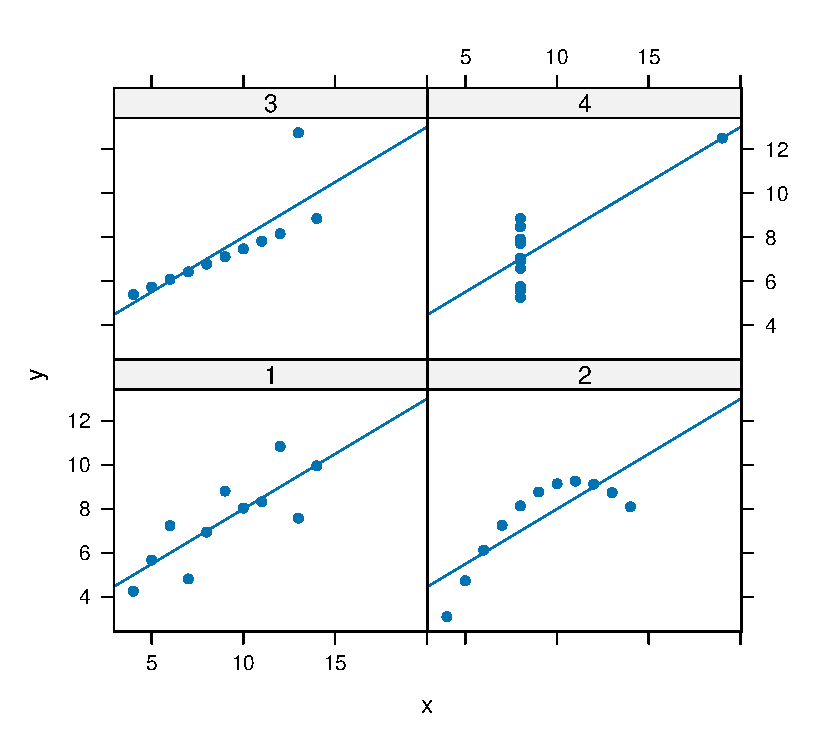
\includegraphics[scale=.6]{../figures/anscombe} 
    \column{.4\textwidth}
  \begin{itemize}
    \item Four data sets by \citet{Anscombe1973} with the same traditional
      statistical properties (mean, variance, correlation, regression line,
      etc.)
    \item Available in R with \texttt{data(anscombe)}
  \end{itemize}
  \end{columns}
\end{frame}

\begin{frame}[fragile]{Assumptions}
\begin{lstlisting}
data(anscombe)

lm1 <- lm(y1 ~ x1, anscombe)
lm2 <- lm(y2 ~ x2, anscombe)
lm3 <- lm(y3 ~ x3, anscombe)
lm4 <- lm(y4 ~ x4, anscombe)

rbind(coef(lm1), coef(lm2), coef(lm3), coef(lm4))

par(mfrow = c(2, 2))
plot(lm1)
plot(lm2)
plot(lm3)
plot(lm4)
\end{lstlisting}
\end{frame}

\begin{frame}{}
  \begin{block}{Exercise}
    \begin{itemize}
      \item Create two vectors $x$ and $y$ with 100 observations each and
        $X \sim N(1,1)$ and $Y \sim N(2,1)$
      \item Create a data frame with variables \texttt{id}, \texttt{group}
        and \texttt{score}. $X$ and $Y$ are your score values
      \item Conduct a $t$ test assuming that $X$ and $Y$ are independent
        having the same variances
      \item Then use the function \texttt{aov()} to compute an analysis of
        variance for these data
      \item Use then function \texttt{lm()} for a linear regression with
        predictor \texttt{group} and dependent variable \texttt{score}
      \item Compare your results
    \end{itemize}
  \end{block}
\end{frame}

\begin{frame}{Extending simple linear regression}
  \begin{tabular}{ll}
    Additional predictors &
      $y = \beta_0 + \beta_1 x_1 + \beta_2 x_2 + \dots +
      \varepsilon$\\
      & \\
    Nonlinear models &
      $\log y = \beta_0 + \beta_1 \log x + \varepsilon$\\
      & \\
    Nonadditive models &
      $y = \beta_0 + \beta_1 x_1 + \beta_2 x_2 + \beta_3
      x_1 x_2 + \varepsilon$\\
      & \\
    Generalized linear models &
      $g(E(y)) = \beta_0 + \beta_1 x$\\
      & \\
    Mixed-effects models &
      $y = \beta_0 + \beta_1 x_1 + \beta_2 time + 
      \upsilon_0 + \upsilon_1 time + \varepsilon$\\
      \dots & \\
  \end{tabular}
\end{frame}


\section{Multiple linear regression}

\begin{frame}{Multiple linear regression}
  \begin{itemize}
    \item Empirical observations consist of tuples for each observation
      unit
\[
  (y_i, x_{i1}, \ldots, x_{ip}) ~~\text{with}~~ i = 1, \ldots, n
\]
and we get the stochastical model
\begin{align*}
  y_i & = \beta_0 + \beta_1 \cdot x_{i1} + \ldots + \beta_p \cdot x_{ip} +
        \varepsilon_i \\
  \varepsilon_i & \sim N (0, \sigma^2)~\text{i.i.d.}
\end{align*}
which transfers to
\[
  y_i \sim N (\mu_i, \sigma^2) ~~\text{with}~~
  \mu_i = \beta_0 + \beta_1 \cdot x_{i1} + \ldots + \beta_p \cdot x_{ip}
\]\vspace{-.7cm}
\item The criterion variable $y$ is always a metric variable, whereas the
  predictor variables $x_1, \ldots, x_p$ can be either metric or
      categorical variables, or both
  \end{itemize}
\end{frame}

\begin{frame}{Overall $F$ test}
  \begin{itemize}
    \item Hypotheses
\begin{align*}
  H_0&\colon~ \beta_1 = \ldots = \beta_p = 0\\
  H_1&\colon~ \beta_j \neq 0 ~\text{ for at least one}~ j \in
  \{1, \ldots, p\}
\end{align*}
\item Test statistic
\[
  F = \frac{R^2}{1 - R^2} \cdot \frac{n - p - 1}{p}
\]
\item Distribution of test statistic assuming $H_0$ is true
\[
  F \sim F(p, n - p - 1)
\]
\item Rejection region
\[
  F > F_{1-\alpha} (p, n - p - 1)
\]
  \end{itemize}
\end{frame}


\begin{frame}{Incremental $F$ test}
  \begin{itemize}
    \item We have two nested models $M_1$ and $M_0$, meaning that $M_0$ is a
      special case of $M_1$ where some parameters $\beta_{M_0,j} = 0$ and
      $\beta_{M_1,j} \neq 0$ and want to test if
  \[
    R_1^2 > R_0^2
  \]
  \item Test statistic
    \[
      F = \frac{R^2_1 - R^2_0}{1 - R^2_1} \cdot \frac{n - q_1}{q_1 - q_0}
    \]
  \item Distribution of test statistic assuming $H_0$ is true
    \[
      F \sim F(q_1 - q_0, n - q_1)
    \]
  \item Rejection region
    \[
      F > F_{1-\alpha} (q_1 - q_0, n - q_1)
    \]
  \end{itemize}
\end{frame}

\begin{frame}{Likelihood ratio test}
  \begin{itemize}
    \item The incremental $F$ test is a special case of the more general
      likelihood ratio test
      \[
        G^2 = 2 \log \frac{L_1}{L_0}
      \]
      where $L_1$ is the likelihood of the more general model and $L_0$ the
      likelihood of the smaller model
    \item The models need to be nested
    \item The test statistic $G^2$ is $\chi^2$ distributed
      \[
        G^2 \sim \chi^2(q_1 - q_0)
      \]
      where $q_1$ and $q_0$ are the number of parameters for the bigger and the
      smaller model, respectively
  \end{itemize}
\end{frame}

\begin{frame}[fragile]{Example: Multiple linear regression}
  \begin{itemize}
    \item We are fitting the following model
\[
y_{ij} = \beta_0 + \beta_1 \cdot x_i + \beta_2 \cdot z_j + \varepsilon_{ij}
\]
with $i = 1 \ldots N$ and $j = 1,2$ for two groups
\item This means that we have one dummy variable for $z$ which takes the
  values 0 and 1
\item Hence, we get the two models
\begin{align*}
y_{i1} & = \beta_0 + \beta_1 \cdot x_i + \beta_2\cdot 0 + \varepsilon_{ij}
= \beta_0 + \beta_1 \cdot x_i + \varepsilon_{ij}\\
y_{i2} & = \beta_0 + \beta_1 \cdot x_i + \beta_2\cdot 1 + \varepsilon_{ij}
= (\beta_0 + \beta_2) + \beta_1 \cdot x_i + \varepsilon_{ij}
\end{align*}
  \end{itemize}
\end{frame}

\begin{frame}[fragile]{Example: Multiple linear regression}
\begin{center}
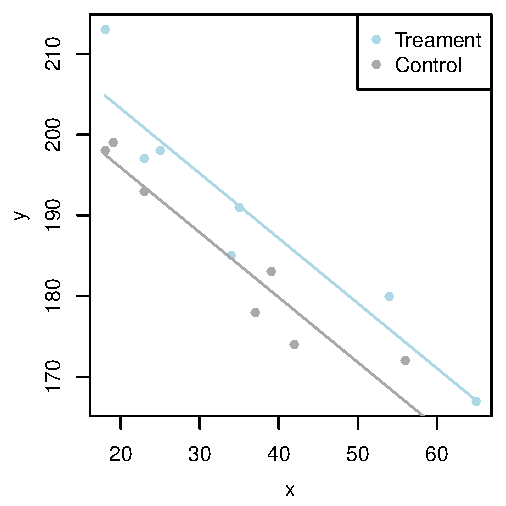
\includegraphics[scale=.8]{../figures/ancova2}
\end{center}
\end{frame}

\begin{frame}[fragile]{Example: Multiple linear regression}
\begin{lstlisting}
dat <- data.frame(
  x = c(18, 23, 25, 35, 65, 54, 34, 56, 72, 19, 23, 42, 18, 39, 37),
  y = c(213, 197, 198, 191, 167, 180, 185, 172, 153, 199, 193, 174,
        198, 183, 178),
  z = rep(c("treatment", "control"), c(7, 8))
)

aggregate(y ~ z, dat, mean)
\end{lstlisting}
\end{frame}

\begin{frame}[fragile]{Example: Multiple linear regression}
  \begin{itemize}
    \item We can now use the parameters to calculate adjusted means for the
      two groups
    \item The observed means are $\bar y_{contr} = 181.25$ and
      $\bar y_{treat} = 190.14$
    \item The adjusted means correspond to
\begin{align*}
  \bar y_{contr} & = \beta_0 & = 181.99\\
  \bar y_{treat} & = \beta_0 + \beta_2 & = 189.30
\end{align*}
These are the means for a value of $x = 0$ which should have a meaningful
interpretation
\item Hence, it might be indicated to center $x$
  \end{itemize}
\end{frame}

\begin{frame}[fragile]{Example: Multiple linear regression}
\begin{lstlisting}
dat$xc <- dat$x - mean(dat$x)

lm2 <- lm(y ~ xc + z, dat)
summary(lm2)

# adjusted means
coef(lm2)[1]
coef(lm2)[1] + coef(lm2)[3]
\end{lstlisting}
\end{frame}

\begin{frame}[fragile]{}
  \begin{block}{Exercise}
    \begin{itemize}
      \item The data set \texttt{cars} contains speed and stopping
        distances of 50 cars
      \item Estimate the regression model
\[
  dist_i = \beta_0 + \beta_1 speed_i + \varepsilon_i
\]\vspace{-.8cm}
      \item How much variance of the stopping distances is explained by
      speed? \item Look at the residuals of the model. Are there any
        systematic deviances?
      \item Now estimate the model
\[
  dist_i = \beta_0 + \beta_1 speed_i + \beta_2 speed^2_i + \varepsilon_i
\]
        Hint: Use \verb+I(speed^2)+ in the model formula in \texttt{R}
      \item Which model fits the data better?
    \end{itemize}
  \end{block}
\end{frame}


\appendix

%\begin{frame}[allowframebreaks]{References}
\begin{frame}{References}
  %\renewcommand{\bibfont}{\footnotesize}
  \printbibliography
  \vfill
\end{frame}

\end{document}

